\documentclass[10pt]{beamer}

\usetheme{Madrid}
\usecolortheme{default}
\setbeamertemplate{navigation symbols}{}
\setbeamersize{text margin left=0.6cm,text margin right=0.6cm}

\usepackage{tikz}
\usetikzlibrary{automata, positioning, arrows.meta, shapes.geometric}
\usepackage{amsmath, amssymb}
\pdfstringdefDisableCommands{\def\translate#1{#1}}

\title{Finite Automata}
\subtitle{Determinism, Nondeterminism, and DFA Minimization}
\author{Computer Science Theory}
\date{Slide Set 2}

\begin{document}

\begin{frame}
  \titlepage
\end{frame}

\begin{frame}{Table of Contents}
  \tableofcontents
\end{frame}

\begin{frame}{Learning Outcomes}
  \small
  By the end of this slide set, you should be able to:
  \begin{itemize}
    \item define DFAs and $\varepsilon$-NFAs formally and trace their
      computations;
    \item design finite automata whose states record exactly the needed
      information about an input prefix;
    \item convert an $\varepsilon$-NFA to an equivalent DFA using subset
      construction;
    \item justify a design or conversion using an invariant;
    \item identify reachable, distinguishable, and equivalent DFA states; and
    \item minimize a DFA using table filling and certify that no further
      merging is possible.
  \end{itemize}
\end{frame}

% ==========================================
% Part 1: Deterministic Finite Automata (DFA)
% ==========================================
\section{Deterministic Finite Automata (DFA)}

\begin{frame}{Part 1: Intuitive Introduction to DFAs}
  \small
  \textbf{Motivating model:} A Simplified Door Controller
  \vspace{0.2cm}
  
  Finite automata are excellent models for computers with an extremely limited amount of memory.
  \pause
  \begin{block}{Example: Automatic Door Controller}
    The controller has states \textbf{OPEN} and \textbf{CLOSED}. Its input
    records whether a person is detected at the front, rear, both sides, or
    neither side. In this toy policy, any detection opens the door;
    no detection closes it. Timing and other physical details are omitted.
  \end{block}
  \pause
  
  \begin{center}
  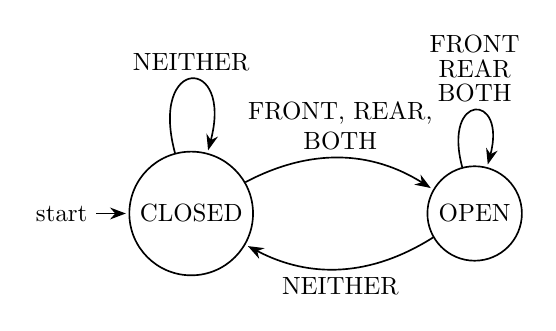
\begin{tikzpicture}[->, >=Stealth, shorten >=1pt, auto, node distance=4cm,
      semithick, scale=0.9, transform shape]
    \node[state, initial] (closed) {CLOSED};
    \node[state] (open) [right of=closed] {OPEN};

    \path (closed) edge [bend left] node {\shortstack{FRONT, REAR,\\BOTH}} (open)
          (closed) edge [loop above] node {NEITHER} (closed)
          (open) edge [bend left] node {NEITHER} (closed)
          (open) edge [loop above] node {\shortstack{FRONT\\REAR\\BOTH}} (open);
  \end{tikzpicture}
  \end{center}
  This diagram models control states. To use such a machine as a
  \emph{language recognizer}, we must also specify which states accept.
\end{frame}

\begin{frame}{Formal Definition of a DFA}
  \small
  To resolve any ambiguities, we require a mathematically precise definition.
  \pause
  \begin{block}{The 5-Tuple Definition}
    A deterministic finite automaton is a 5-tuple
    $M=(Q,\Sigma,\delta,q_0,F)$, where:
    \begin{enumerate}
        \item $Q$ is a finite, nonempty set of states,
        \item $\Sigma$ is a finite input alphabet,
        \item $\delta: Q \times \Sigma \rightarrow Q$ is the transition function,
        \item $q_0 \in Q$ is the start state, and
        \item $F \subseteq Q$ is the set of accept states.
    \end{enumerate}
  \end{block}
  \pause
  \vspace{0.2cm}
  \textbf{Crucial detail:} $\delta$ is total. For every $q\in Q$ and
  $a\in\Sigma$, exactly one transition $\delta(q,a)$ is defined.
\end{frame}

\begin{frame}{Extended Transition Function}
  \small
  The transition function $\delta$ strictly handles single symbols. To describe the processing of entire strings, it is convenient to introduce the extended transition function $\delta^* : Q \times \Sigma^* \rightarrow Q$.
  \pause
  \begin{block}{Recursive Definition of $\delta^*$}
    We define $\delta^*$ recursively as follows:
    \begin{enumerate}
        \item $\delta^*(q, \varepsilon) = q$.
        \item $\delta^*(q, wa) = \delta(\delta^*(q,w), a)$  for all $w \in \Sigma^*$ and $a \in \Sigma$.
    \end{enumerate}
  \end{block}
  \pause
  \vspace{0.2cm}
  \textbf{Language recognized by $M$:}
  \[
    L(M)=\{w\in\Sigma^*: \delta^*(q_0,w)\in F\}.
  \]
  A language is \textbf{regular} if it is recognized by some DFA.
  \pause
  A useful composition law (induction on $|v|$) is
  \[
    \delta^*(q,uv)=\delta^*(\delta^*(q,u),v).
  \]
  Reading $uv$ means reading $u$ first, then continuing with $v$.
\end{frame}

\begin{frame}{Reading a DFA: Runs and Boundary Cases}
  \small
  For $w=a_1\cdots a_m$, the unique run is $r_0,\ldots,r_m$, where
  \[
    r_0=q_0,\qquad r_i=\delta(r_{i-1},a_i)\quad(1\le i\le m).
  \]
  The machine accepts exactly when $r_m\in F$.
  \pause
  \begin{itemize}
    \item Visiting an accepting state midway is not enough; consume the
      \emph{entire} input before deciding.
    \item The empty word consumes no symbols:
      $\varepsilon\in L(M)$ iff $q_0\in F$.
    \item $F=\emptyset$ is allowed and gives $L(M)=\emptyset$.
      If $F=Q$, then $L(M)=\Sigma^*$.
  \end{itemize}
  \pause
  \begin{block}{How to read the drawing}
    An incoming arrow marks the start; a double circle marks acceptance.
    An edge labeled $0,1$ abbreviates two transitions, not the word $01$.
    A DFA has no $\varepsilon$-moves; $\varepsilon$ is not an input symbol.
  \end{block}
\end{frame}

% ==========================================
% Part 2: Designing DFAs
% ==========================================
\section{Designing DFAs}

\begin{frame}{A Design Method: What Must the State Remember?}
  \small
  \begin{enumerate}
    \item Give each state a precise meaning about the prefix read so far.
    \item Choose the state whose meaning holds for the empty prefix.
    \item For every state and symbol, update that meaning in one step.
    \item Mark states whose meaning guarantees the required condition
      \emph{if the input ends now}.
    \item Test boundary words, then prove the state meanings by induction.
  \end{enumerate}
  \pause
  \begin{block}{Reusable correctness proof}
    \textbf{Base:} the invariant holds before reading input.
    \textbf{Step:} each transition preserves the invariant after one symbol.
    \textbf{Conclusion:} the accepting states correspond exactly to the
    desired words. This proves both soundness and completeness.
  \end{block}
  Typical memories: a count modulo $k$, progress through a required prefix,
  or the longest relevant suffix. Avoid storing irrelevant history.
\end{frame}

\begin{frame}{Designing DFAs: Case Study 1}
  \small
  \textbf{Goal:} Construct a DFA accepting all strings over $\{0,1\}$ with an \textbf{odd number of 1s}.
  \pause
  \vspace{0.2cm}
  
  \textit{Thought Process:} We don't need to remember the entire string. We only need to remember whether the number of 1s seen so far is even or odd.
  \pause
  
  \begin{center}
  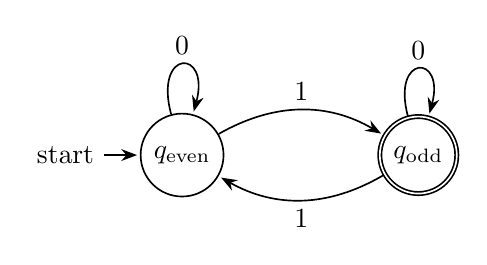
\begin{tikzpicture}[->, >=Stealth, shorten >=1pt, auto, node distance=3cm, semithick]
    \node[state, initial] (qeven) {$q_{\mathrm{even}}$};
    \node[state, accepting] (qodd) [right of=qeven] {$q_{\mathrm{odd}}$};

    \path (qeven) edge [bend left] node {1} (qodd)
          (qeven) edge [loop above] node {0} (qeven)
          (qodd) edge [bend left] node {1} (qeven)
          (qodd) edge [loop above] node {0} (qodd);
  \end{tikzpicture}
  \end{center}
  
  \begin{itemize}
      \item \textbf{States:} $Q = \{q_{\mathrm{even}},q_{\mathrm{odd}}\}$.
      \item \textbf{Start state:} $q_{\mathrm{even}}$ (zero 1s is even).
      \item \textbf{Accepting states:} $F=\{q_{\mathrm{odd}}\}$.
  \end{itemize}
\end{frame}

\begin{frame}{Designing DFAs: Case Study 2 \& Trap States}
  \footnotesize
  \textbf{Goal:} Construct a DFA over $\{a,b\}$ accepting strings beginning
  with the prefix $ab$.
  \pause
  \begin{center}
  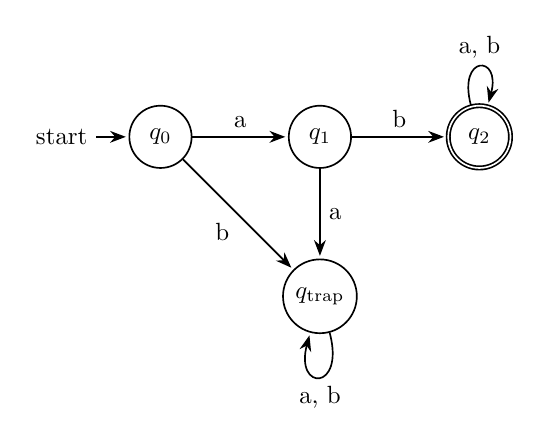
\begin{tikzpicture}[->, >=Stealth, shorten >=1pt, auto, node distance=2.25cm,
      semithick, scale=0.9, transform shape]
    \node[state, initial] (q0) {$q_0$};
    \node[state] (q1) [right of=q0] {$q_1$};
    \node[state, accepting] (q2) [right of=q1] {$q_2$};
    \node[state] (qt) [below of=q1] {$q_{\mathrm{trap}}$};

    \path (q0) edge node {a} (q1)
          (q0) edge node [swap] {b} (qt)
          (q1) edge node {b} (q2)
          (q1) edge node {a} (qt)
          (q2) edge [loop above] node {a, b} (q2)
          (qt) edge [loop below] node {a, b} (qt);
  \end{tikzpicture}
  \end{center}
  \pause
  \begin{alertblock}{Teacher's Corner: The Trap State}
    A DFA may not simply omit a transition: $\delta$ must be total. Once the
    required prefix becomes impossible, the machine enters a nonaccepting
    \textbf{rejecting sink} (trap) state and remains there. A sink has
    self-loops on every symbol; a sink can also be accepting, as $q_2$ is here.
  \end{alertblock}
\end{frame}

\begin{frame}{Designing DFAs: Case Study 3}
  \small
  \textbf{Goal:} Construct a DFA over $\{0,1\}$ recognizing strings that do
  not contain the substring $001$.
  \pause
  \vspace{0.2cm}
  
  \textit{Strategy:} Track the longest suffix of the input that is also a
  prefix of $001$. Once $001$ occurs, enter a rejecting trap state.
  In particular, after $000$ the relevant suffix is still $00$.
  
  \begin{center}
  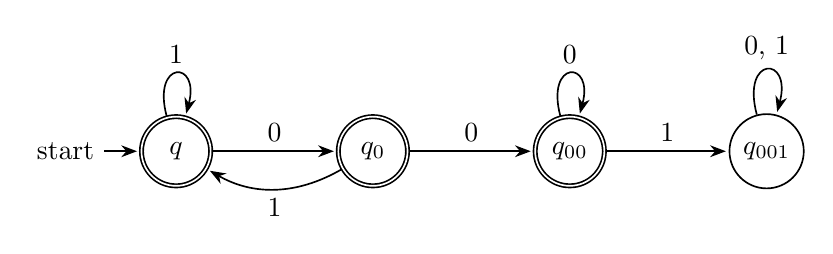
\begin{tikzpicture}[->, >=Stealth, shorten >=1pt, auto, node distance=2.5cm, semithick]
    \node[state, initial, accepting] (q) {$q$};
    \node[state, accepting] (q0) [right of=q] {$q_0$};
    \node[state, accepting] (q00) [right of=q0] {$q_{00}$};
    \node[state] (q001) [right of=q00] {$q_{001}$};

    \path (q) edge [loop above] node {1} (q)
          (q) edge node {0} (q0)
          (q0) edge [bend left] node {1} (q)
          (q0) edge node {0} (q00)
          (q00) edge [loop above] node {0} (q00)
          (q00) edge node {1} (q001)
          (q001) edge [loop above] node {0, 1} (q001);
  \end{tikzpicture}
  \end{center}
  The states $q,q_0,q_{00}$ are accepting because the forbidden pattern has
  not yet appeared. State $q_{001}$ is a rejecting trap state.
\end{frame}

% ==========================================
% Part 3: Nondeterministic Finite Automata (NFA)
% ==========================================
\section{Nondeterministic Finite Automata (NFA)}

\begin{frame}{Part 3: Introduction to Nondeterminism}
  \small
  \textbf{Self-Study Header:} The Power of Choice
  \vspace{0.2cm}
  
  Nondeterminism allows several possible next states. A DFA is a special
  case: replace each successor $q$ by the singleton set $\{q\}$.
  \pause
  \begin{itemize}
      \item \textbf{Branching model:} We may imagine the machine exploring all
        permitted paths; this is a mathematical model, not literal hardware
        duplication.
      \item \textbf{Acceptance:} The machine accepts if \textit{at least one} branch reaches an accept state at the end of the input.
      \item \textbf{Empty transitions:} In the $\varepsilon$-NFA model,
        a move labeled $\varepsilon$ (or $\lambda$) changes state without
        consuming input. Taking such a move is a possible choice, not an
        obligation to follow it before all other moves.
  \end{itemize}
\end{frame}

\begin{frame}{Formal Definition of an NFA}
  \small
  An $\varepsilon$-NFA is a tuple $N=(Q,\Sigma,\delta,q_0,F)$.
  The components $Q,\Sigma,q_0,F$ have the same meanings as for a DFA.
  We use Sipser's convention of allowing $\varepsilon$-moves in an NFA;
  other texts distinguish an NFA from an $\varepsilon$-NFA.
  \pause
  \begin{block}{The Transition Function $\delta$}
    Let $\Sigma_\varepsilon = \Sigma \cup \{\varepsilon\}$.
    The transition function takes a state and an input symbol or the empty string and produces the \textbf{set} of possible next states.
    
    \[
      \delta:Q\times\Sigma_\varepsilon\longrightarrow\mathcal{P}(Q).
    \]
  \end{block}
  \pause
  \vspace{0.3cm}
  Here, $\mathcal{P}(Q)$ (or $2^Q$) is the power set of $Q$. Since the output is a set of states:
  \begin{itemize}
      \item It can return one state: $\{q_1\}$.
      \item It can return several states: $\{q_1,q_2\}$.
      \item It can return $\emptyset$, meaning no path continues by that move.
  \end{itemize}
  Every unspecified transition has value $\emptyset$. An NFA without
  $\varepsilon$-moves has $\delta(q,\varepsilon)=\emptyset$ for all $q$.
\end{frame}

\begin{frame}{Computing Epsilon-Closure, Even with Cycles}
  \small
  For $R\subseteq Q$, let
  \[
    E(R)=\{q:\text{some state in }R\text{ reaches }q
                    \text{ using only }\varepsilon\text{-moves}\}.
  \]
  Zero moves are allowed, so $R\subseteq E(R)$ and $E(\emptyset)=\emptyset$.
  \begin{center}
    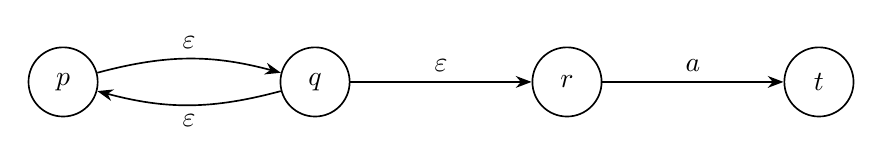
\begin{tikzpicture}[->,>=Stealth,auto,semithick,node distance=2.3cm]
      \node[state] (p) {$p$};
      \node[state,right=of p] (q) {$q$};
      \node[state,right=of q] (r) {$r$};
      \node[state,right=of r] (t) {$t$};
      \path (p) edge[bend left=15] node {$\varepsilon$} (q)
        (q) edge[bend left=15] node {$\varepsilon$} (p)
        (q) edge node {$\varepsilon$} (r)
        (r) edge node {$a$} (t);
    \end{tikzpicture}
  \end{center}
  \pause
  $E(\{p\})=\{p,q,r\}$; do not cross the $a$-edge.
  Start a worklist with $R$ and add unseen $\varepsilon$-successors until
  none remain. Mark each visited state, so cycles do not cause nontermination.
  \begin{block}{Acceptance means existence of a finite successful path}
    An infinite $\varepsilon$-loop is not an accepting computation. It also
    does not prevent acceptance if another finite path consumes the input
    and ends in an accepting state.
  \end{block}
\end{frame}

\begin{frame}{NFA Example}
  \small
  \textbf{Goal:} Accept strings containing either $101$ or $11$ as a
  substring.
  \pause
  \vspace{0.2cm}
  
  \begin{center}
  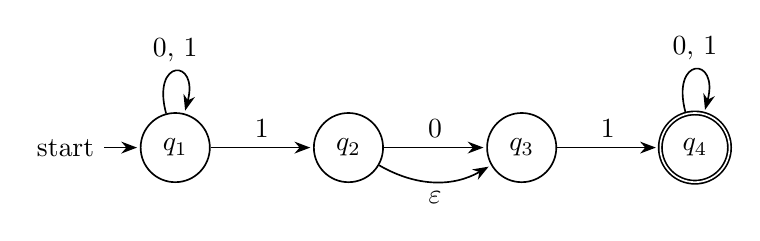
\begin{tikzpicture}[->, >=Stealth, shorten >=1pt, auto, node distance=2.2cm, semithick]
    \node[state, initial] (q1) {$q_1$};
    \node[state] (q2) [right of=q1] {$q_2$};
    \node[state] (q3) [right of=q2] {$q_3$};
    \node[state, accepting] (q4) [right of=q3] {$q_4$};

    \path (q1) edge [loop above] node {0, 1} (q1)
          (q1) edge node {1} (q2)
          (q2) edge node {0} (q3)
          (q2) edge [bend right] node [swap] {$\varepsilon$} (q3)
          (q3) edge node {1} (q4)
          (q4) edge [loop above] node {0, 1} (q4);
  \end{tikzpicture}
  \end{center}
  \pause
  \textbf{Why is this an NFA?}
  \begin{enumerate}
      \item From $q_1$, reading $1$ may remain in $q_1$ or move to $q_2$.
      \item The path $q_2\xrightarrow{0}q_3\xrightarrow{1}q_4$ completes
        the substring $101$.
      \item Alternatively, $q_2\xrightarrow{\varepsilon}q_3$ consumes no
        symbol, so the next $1$ completes the substring $11$.
  \end{enumerate}
\end{frame}

\begin{frame}{Simulating an NFA: Sets, Not a Single Guess}
  \small
  Let $R_w$ be all states reachable after consuming $w$, allowing
  $\varepsilon$-moves before, between, and after input symbols. Then
  \[
    R_\varepsilon=E(\{q_0\}),\qquad
    R_{wa}=E\!\left(\bigcup_{q\in R_w}\delta(q,a)\right).
  \]
  Accept exactly when $R_w\cap F\ne\emptyset$.
  \pause
  For the preceding NFA for containing $101$ or $11$, the start is $q_1$:
  \[
    \begin{array}{c|l}
      \text{prefix} & \text{reachable set, after closure}\\
      \hline
      \varepsilon & \{q_1\}\\
      1 & \{q_1,q_2,q_3\}\\
      10 & \{q_1,q_3\}\\
      101 & \{q_1,q_2,q_3,q_4\}
    \end{array}
  \]
  \pause
  The last set contains $q_4$, so $101$ is accepted. One unsuccessful path
  cannot establish rejection: \emph{every} path must fail to accept.
  If the reachable set becomes empty, it stays empty on further input.
\end{frame}

% ==========================================
% Part 4: Equivalence of DFA and NFA
% ==========================================
\section{Equivalence of DFA and NFA}

\begin{frame}{Part 4: Equivalence Theorem}
  \small
  \textbf{Theorem:} Every nondeterministic finite automaton has an equivalent deterministic finite automaton.
  \vspace{0.2cm}
  
  \pause
  This is a surprising but highly useful result. It tells us that adding nondeterminism \textit{does not increase} the computational power of a finite automaton—they both recognize exactly the class of regular languages.
  \pause
  
  \begin{block}{Proof Idea: The Subset Construction Algorithm}
    If the NFA has $k$ states, a DFA state records the set of NFA states
    reachable after the prefix read so far. At most $2^k$ subsets exist, though
    usually only some are reachable.
  \end{block}
\end{frame}

\begin{frame}{The Subset Construction Algorithm}
  \small
  Let $N = (Q, \Sigma, \delta_N, q_0, F_N)$ be an NFA. We build an equivalent DFA $M = (Q', \Sigma, \delta_M, q_0', F')$.
  \pause
  \begin{itemize}
      \item \textbf{States:} Begin with $Q'=\mathcal{P}(Q)$ conceptually, then
        retain only subsets reachable from the start subset.
      \pause
      \item \textbf{$\varepsilon$-closure:} $E(R)$ contains the states reachable
        from $R$ using zero or more $\varepsilon$-moves.
      \pause
      \item \textbf{Start State ($q_0'$):} $q_0' = E(\{q_0\})$. We begin by calculating the $\varepsilon$-closure of the NFA's start state.
      \pause
      \item \textbf{Transition function:} For $R\in Q'$ and $a\in\Sigma$,
      \[
        \delta_M(R,a)=E\!\left(\bigcup_{r\in R}\delta_N(r,a)\right).
      \]
      \pause
      \item \textbf{Accepting states:}
        $F'=\{R\in Q':R\cap F_N\neq\emptyset\}$.
  \end{itemize}
  \begin{exampleblock}{Correctness Invariant}
    After reading $w$, the DFA is in exactly the set of NFA states reachable
    from $q_0$ by paths whose non-$\varepsilon$ labels spell $w$.
  \end{exampleblock}
\end{frame}

\begin{frame}{Worked Example: NFA to DFA}
  \small
  Consider this $\varepsilon$-NFA over $\{a,b\}$, with states $1,2,3$:
  \begin{center}
  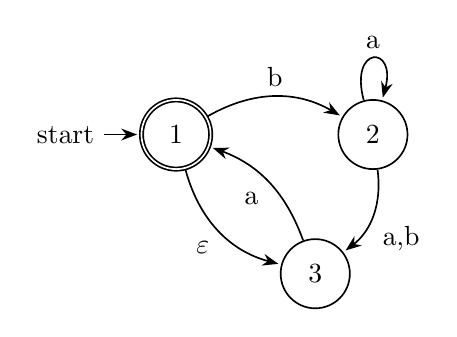
\begin{tikzpicture}[->, >=Stealth, shorten >=1pt, auto, node distance=2.5cm, semithick]
    \node[state, initial, accepting] (1) {1};
    \node[state] (2) [right of=1] {2};
    \node[state] (3) [below right of=1] {3};

    \path (1) edge [bend left] node {b} (2)
          (1) edge [bend right] node [swap] {$\varepsilon$} (3)
          (2) edge [loop above] node {a} (2)
          (2) edge [bend left] node {a,b} (3)
          (3) edge [bend right=25] node {a} (1);
  \end{tikzpicture}
  \end{center}
  \pause
  \textbf{Start the subset construction:}
  \begin{itemize}
      \item \textbf{Start State:} $E(\{1\}) = \{1, 3\}$ (since $1 \xrightarrow{\varepsilon} 3$).
      \item \textbf{From $\{1,3\}$ on $a$:}
      $\delta_N(1, a) = \emptyset$, $\delta_N(3, a) = \{1\}$. 
      Closure $E(\{1\}) = \{1,3\}$. So, $\delta_M(\{1,3\}, a) = \{1,3\}$.
      \item \textbf{From $\{1,3\}$ on $b$:}
      $\delta_N(1, b) = \{2\}$, $\delta_N(3, b) = \emptyset$.
      Closure $E(\{2\}) = \{2\}$. So, $\delta_M(\{1,3\}, b) = \{2\}$.
  \end{itemize}
\end{frame}

\begin{frame}[label=subset-table]{Worked Example: NFA to DFA (Completed)}
  \small
  Continuing until no new subset appears gives the following six reachable
  DFA states.
  \[
  \begin{array}{c@{\qquad}cc@{\qquad}c}
    \text{DFA state} & a & b & \text{accepting?}\\[2pt]
    A=\{1,3\}     & A & B & \checkmark\\
    B=\{2\}       & C & D & \\
    C=\{2,3\}     & E & D & \\
    D=\{3\}       & A & \varnothing & \\
    E=\{1,2,3\}   & E & C & \checkmark\\
    \varnothing    & \varnothing & \varnothing &
  \end{array}
  \]
  \pause
  $A$ is the start state. Reachability witnesses for the rows are
  $\varepsilon,b,ba,bb,baa,bbb$, respectively.
  Exactly $A$ and $E$ contain the NFA's accepting state $1$.
  \begin{block}{Stop when the reachable-subset worklist is empty}
    Process every new subset on every alphabet symbol, reusing a subset
    already seen. Only six of the $2^3=8$ possible subsets occur here.
    The empty subset is a single DFA state, not an omitted transition.
  \end{block}
  \hyperlink{subset-diagram}{\beamerbutton{Optional state diagram in appendix}}
\end{frame}


% ==========================================
% Part 5: DFA Minimization
% ==========================================
\section{DFA Minimization (State Reduction)}

\begin{frame}{Part 5: Motivation for State Reduction}
  \small
  \textbf{Self-Study Header:} Finding the Smallest Equivalent DFA
  \vspace{0.2cm}
  
  For a given regular language, there are infinitely many DFAs that recognize it. For practical applications (like compiling and text searching), we want the \textbf{minimal} DFA—the one with the fewest possible states.
  
  \pause
  \begin{block}{Indistinguishable States}
    States $p$ and $q$ are \textbf{equivalent} (indistinguishable), written
    $p\equiv q$, if for every suffix $w\in\Sigma^*$,
    \[
      \delta^*(p,w)\in F
      \iff
      \delta^*(q,w)\in F.
    \]
    Otherwise they are distinguishable; any witnessing $w$ is a
    \textbf{distinguishing string}.
  \end{block}
  \pause
  Equivalent reachable states represent the same future behavior and may be
  merged without changing the recognized language.
\end{frame}

\begin{frame}{Before Minimizing: Reachability Is Not Equivalence}
  \small
  A state $q$ is \textbf{reachable} if $\delta^*(q_0,w)=q$ for some word $w$.
  Find reachable states by graph search from $q_0$, following every symbol.
  \pause
  \begin{itemize}
    \item Remove unreachable states: no input run visits them.
    \item A reachable nonaccepting state may still lead to acceptance;
      being nonaccepting does not make a state useless.
    \item A \textbf{dead} state has no accepting continuation. Reachable
      dead states all have the same future behavior, so merge them into
      one rejecting sink rather than deleting them from a complete DFA.
  \end{itemize}
  \pause
  \begin{exampleblock}{The prefix-$ab$ machine}
    Its trap is reached by $b$. Deleting the trap would leave the start's
    $b$-transition undefined. The intermediate state reached by $a$ is not
    dead: suffix $b$ leads to acceptance.
  \end{exampleblock}
  For a fixed alphabet, the minimal complete DFA for $\emptyset$ has one
  nonaccepting sink; the minimal one for $\Sigma^*$ has one accepting sink.
\end{frame}

\begin{frame}{The Table-Filling Algorithm}
  \small
  Work with a complete DFA. A marked pair has a distinguishing suffix.
  
  \begin{enumerate}
      \item \textbf{Initialize:} Remove all unreachable states.
      \pause
      \item \textbf{Initialize the table:} List every unordered pair
        $\{p,q\}$ and mark pairs with exactly one accepting state.
      \pause
      \item \textbf{Iterate:} For every unmarked pair $(p, q)$ and every symbol $a \in \Sigma$:
      \begin{itemize}
          \item Compute $r = \delta(p, a)$ and $s = \delta(q, a)$.
          \item If $r\ne s$ and $\{r,s\}$ is marked, mark $\{p,q\}$.
            If $w$ witnesses the successor pair, $aw$ witnesses this pair.
      \end{itemize}
      \pause
      \item \textbf{Terminate:} Repeat step 3 until a full pass makes no new marks.
      \item \textbf{Merge:} The remaining unmarked pairs are equivalent;
        collapse each equivalence class to one state.
  \end{enumerate}
  \begin{exampleblock}{Minimal-DFA Theorem}
    After unreachable states are removed and equivalent states are merged, the
    resulting complete DFA is minimal and is unique up to renaming states
    (over the same alphabet).
  \end{exampleblock}
\end{frame}

\begin{frame}{Minimization Example: Start with a Transition Table}
  \small
  Use the DFA below, with start $q_0$ and $F=\{q_2,q_4\}$.
  \[
    \begin{array}{c|cc|c}
      \text{state} & 0 & 1 & \text{a word reaching it}\\
      \hline
      q_0 & q_1 & q_3 & \varepsilon\\
      q_1 & q_2 & q_4 & 0\\
      q_2 & q_1 & q_4 & 00\\
      q_3 & q_2 & q_4 & 1\\
      q_4 & q_4 & q_4 & 01
    \end{array}
  \]
  Every state is reachable, so none can be removed at the first step.
  \pause
  \begin{block}{Predict before marking}
    $q_1$ and $q_3$ have identical successors and are both nonaccepting.
    They are equivalent. But $q_2$ and $q_4$, although both accepting,
    differ after input $0$: $q_2$ rejects it and $q_4$ accepts it.
  \end{block}
  Identical transition rows with matching acceptance are sufficient for
  equivalence, but not necessary. Table filling handles the general case.
\end{frame}

\begin{frame}{Minimization Example: Marking the Pairs}
  \small
  Put a distinguishing suffix in each marked cell. Initially, $\varepsilon$
  marks pairs with exactly one accepting state.
  \[
    \begin{array}{c|cccc}
      q_1 & \uncover<2->{0}\\
      q_2 & \varepsilon & \varepsilon\\
      q_3 & \uncover<2->{0} & \uncover<2->{\sim} & \varepsilon\\
      q_4 & \varepsilon & \varepsilon & \uncover<2->{0} & \varepsilon\\
      \hline
          & q_0 & q_1 & q_2 & q_3
    \end{array}
  \]
  \pause
  The three new marks have witness $0$:
  \[
    \begin{aligned}
      (q_0,q_1)&\xrightarrow{0}(q_1,q_2),&
      (q_0,q_3)&\xrightarrow{0}(q_1,q_2),\\
      (q_2,q_4)&\xrightarrow{0}(q_1,q_4).&&
    \end{aligned}
  \]
  Their successor pairs were already marked by $\varepsilon$.
  \begin{block}{The fixed point}
    No further marks are possible. The cell $\sim$ remains unmarked:
    only $q_1\equiv q_3$. A blank cell means equivalent only
    \emph{after} the algorithm has reached its fixed point.
  \end{block}
\end{frame}

\begin{frame}{Minimization Example: The Quotient DFA}
  \small
  Create one state per equivalence class:
  \[
    A=\{q_0\},\quad B=\{q_1,q_3\},\quad
    C=\{q_2\},\quad D=\{q_4\}.
  \]
  Start at $A$; accept at $C,D$. Each transition goes to the class of the
  old successor: $\delta_{\min}([q],a)=[\delta(q,a)]$.
  \begin{center}
    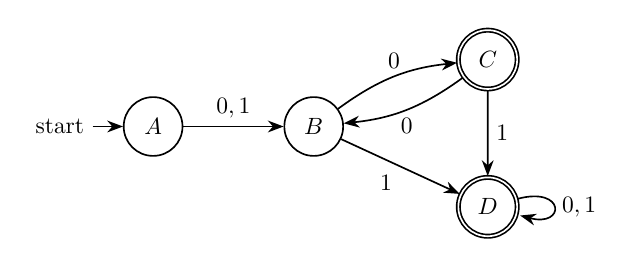
\begin{tikzpicture}[->,>=Stealth,auto,semithick,scale=0.85,transform shape]
      \node[state,initial] (A) at (0,0) {$A$};
      \node[state] (B) at (2.4,0) {$B$};
      \node[state,accepting] (C) at (5,1.0) {$C$};
      \node[state,accepting] (D) at (5,-1.2) {$D$};
      \path (A) edge node {$0,1$} (B)
        (B) edge[bend left=15] node[above] {$0$} (C)
        (B) edge node[below left] {$1$} (D)
        (C) edge[bend left=15] node[below] {$0$} (B)
        (C) edge node[right] {$1$} (D)
        (D) edge[loop right] node {$0,1$} (D);
    \end{tikzpicture}
  \end{center}
  \pause
  \textbf{Minimality certificate.} All four states are reachable.
  $\varepsilon$ distinguishes every accepting/nonaccepting pair;
  $0$ distinguishes $A$ from $B$ and $C$ from $D$.
  Thus no two reachable states have the same future behavior.
\end{frame}

% ==========================================
% Pedagogical Enhancements
% ==========================================
\section{Exercises and Review}

\begin{frame}{Checkpoint Exercises}
  \small
  \begin{enumerate}
      \item \textbf{DFA Design:} Draw the state diagram of a DFA over the alphabet $\Sigma = \{0, 1\}$ that recognizes the language: $\{w \mid w \text{ contains at least two 0s}\}$.
      \vspace{0.5cm}
      \item \textbf{NFA Trace:} Consider an NFA with states $\{q_0, q_1, q_2\}$. The start state is $q_0$.
      \begin{itemize}
          \item $\delta(q_0, \varepsilon) = \{q_1\}$
          \item $\delta(q_1, \varepsilon) = \{q_2\}$
          \item $\delta(q_0, a) = \{q_0\}$
      \end{itemize}
      What is the $\varepsilon$-closure of the start state $q_0$? That is, find $E(\{q_0\})$.
      \vspace{0.5cm}
      \item \textbf{Minimization Logic:} A complete DFA has exactly two
        reachable states, one accepting and one nonaccepting. Can these states
        be merged? Give a distinguishing string.
  \end{enumerate}
\end{frame}

\begin{frame}{Common Mistakes and Quick Diagnostic Questions}
  \small
  \begin{itemize}
    \item \textbf{Missing DFA edge:} is there exactly one successor for
      every state-symbol pair?
    \item \textbf{Premature acceptance:} what state or state set remains
      after the \emph{last} input symbol?
    \item \textbf{Incorrect NFA rejection:} did all possible computations
      fail, or only the one you happened to follow?
    \item \textbf{Lost empty moves:} did you close the initial set and every
      set obtained after consuming a symbol?
    \pause
    \item \textbf{Wrong merge:} do two states agree for every suffix, not
      merely on being accepting now?
    \item \textbf{Wrong deletion:} is a state unreachable, or merely unable
      to accept? A complete DFA must retain a destination for every input.
    \item \textbf{Premature minimality:} have you removed unreachable states
      and continued marking until no new pair is distinguishable?
  \end{itemize}
\end{frame}

\begin{frame}{Summary: Design, Simulate, Convert, Minimize}
  \small
  \begin{itemize}
    \item A DFA has one run per word. Its current state summarizes the
      relevant input history; acceptance is tested at the end.
    \pause
    \item An NFA accepts if some finite path consumes the whole word and
      finishes in an accepting state. State-set simulation accounts for
      every possible path, including $\varepsilon$-moves.
    \pause
    \item Subset construction turns those state sets into DFA states,
      preserving the language but possibly increasing the representation size.
    \pause
    \item Minimization discards unreachable states and merges states with
      identical future acceptance behavior. Distinguishing suffixes certify
      which states must remain separate.
  \end{itemize}
  \begin{block}{Next steps}
    Slide Set~3 connects finite automata with regular expressions and regular
    grammars. Slide Set~4 studies closure, decision properties, and the
    limits of finite memory. The appendix here supplies optional depth.
  \end{block}
\end{frame}

\appendix
\section{Appendix: Solutions and Optional Theory}

\begin{frame}{Appendix Guide: Choose a Teaching Route}
  \small
  The main lecture retains the definitions, core state-design examples,
  subset-construction table, and complete marking/minimization sequence.
  \begin{block}{Supplementary material moved out of the main lecture}
    The detailed parity proof; the additional suffix-$01$ example; the
    determinized state diagram; and the further-practice sheet are now here.
    The table and its optional diagram have navigation links.
  \end{block}
  \begin{itemize}
    \item \textbf{Practice route:} worked solutions, binary addition and
      comparison, and the shortest accepted-word challenge.
    \item \textbf{Proof route:} subset correctness, epsilon removal,
      marking correctness, partition refinement, and Myhill--Nerode.
    \item \textbf{Enrichment route:} double-reversal minimization,
      exponential state gaps, NFA lower bounds, and algorithmic costs.
  \end{itemize}
  These are optional extensions, not an additional required lecture.
  Closure properties and pumping arguments are left to Slide Set~4.
\end{frame}

\subsection{Supplementary Examples}

\begin{frame}{A Trace and a Proof: Odd Number of Ones}
  \small
  Recall the parity DFA: start even, toggle on $1$, and stay on $0$.
  Only the odd state accepts. Trace $0110$:
  \[
    \begin{array}{c|ccccc}
      \text{prefix read} & \varepsilon & 0 & 01 & 011 & 0110\\
      \hline
      \text{state} & q_{\mathrm{even}} & q_{\mathrm{even}} & q_{\mathrm{odd}}
        & q_{\mathrm{even}} & q_{\mathrm{even}}
    \end{array}
  \]
  The full word is rejected, despite the earlier visit to $q_{\mathrm{odd}}$.
  \pause
  \begin{block}{Inductive invariant}
    After reading $w$, the state is $q_{\mathrm{even}}$ iff $|w|_1$ is even,
    and $q_{\mathrm{odd}}$ iff $|w|_1$ is odd. Here $|w|_1$ counts the $1$'s.
    \begin{itemize}
      \item \textbf{Base:} $w=\varepsilon$ has zero $1$'s, so the start is correct.
      \item \textbf{Step:} appending $0$ preserves parity; appending $1$ flips it.
        The transitions implement exactly these updates.
    \end{itemize}
  \end{block}
  \pause
  Since only the odd state accepts, the invariant proves that the DFA accepts
  exactly the intended language, for every input length.
\end{frame}

\begin{frame}{Designing DFAs: Ending in 01 Is Different}
  \small
  \textbf{Goal:} Accept binary words whose final two symbols are $01$.
  A previously matched $01$ may cease to be a suffix after more input.
  \begin{center}
    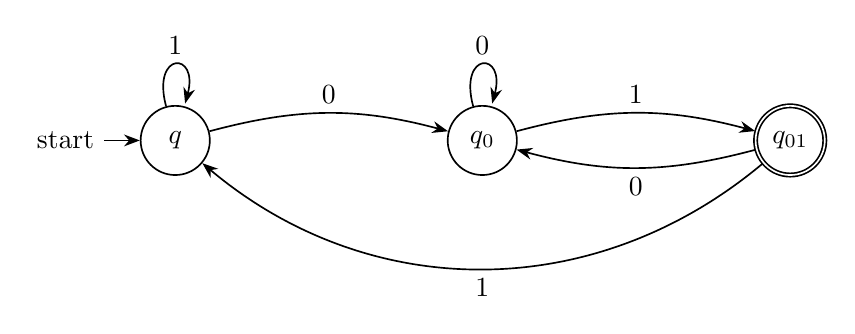
\begin{tikzpicture}[->,>=Stealth,auto,semithick,node distance=3cm]
      \node[state,initial] (q) {$q$};
      \node[state,right=of q] (q0) {$q_0$};
      \node[state,accepting,right=of q0] (q01) {$q_{01}$};
      \path (q) edge[loop above] node {$1$} (q)
        (q) edge[bend left=15] node {$0$} (q0)
        (q0) edge[loop above] node {$0$} (q0)
        (q0) edge[bend left=15] node {$1$} (q01)
        (q01) edge[bend left=15] node {$0$} (q0)
        (q01) edge[bend left=40] node[below] {$1$} (q);
    \end{tikzpicture}
  \end{center}
  \pause
  The states remember the longest suffix that is a prefix of $01$:
  $\varepsilon$, $0$, or $01$. Test $01$ (accept), $010$ (reject), and
  $0101$ (accept).
  \begin{alertblock}{Three different specifications}
    \emph{Begins with}, \emph{contains}, and \emph{ends with} are not
    interchangeable. Once a required substring occurs, success persists;
    a suffix condition must be checked again after every new symbol.
  \end{alertblock}
\end{frame}

\begin{frame}[label=subset-diagram]{Worked Example: The Determinized State Diagram}
  \small
  This implements the main lecture's subset table; start at $A$.
  Here $A=\{1,3\}$, $B=\{2\}$, $C=\{2,3\}$, $D=\{3\}$,
  and $E=\{1,2,3\}$.
  \hyperlink{subset-table}{\beamerbutton{Return to table}}
  \begin{center}
  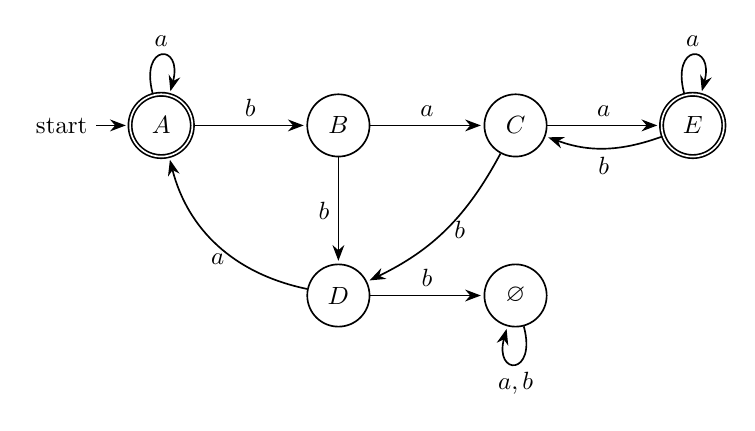
\begin{tikzpicture}[->, >=Stealth, shorten >=1pt, auto, semithick,
      scale=0.9, transform shape]
    \node[state, initial, accepting] (A) at (0,1.4) {$A$};
    \node[state] (B) at (2.5,1.4) {$B$};
    \node[state] (C) at (5,1.4) {$C$};
    \node[state, accepting] (E) at (7.5,1.4) {$E$};
    \node[state] (D) at (2.5,-1.0) {$D$};
    \node[state] (O) at (5,-1.0) {$\varnothing$};

    \path (A) edge[loop above] node {$a$} (A)
          (A) edge node {$b$} (B)
          (B) edge node {$a$} (C)
          (B) edge node[left] {$b$} (D)
          (C) edge node {$a$} (E)
          (C) edge[bend left=18] node[right] {$b$} (D)
          (D) edge[bend left=32] node[below] {$a$} (A)
          (D) edge node {$b$} (O)
          (E) edge[loop above] node {$a$} (E)
          (E) edge[bend left=20] node[below] {$b$} (C)
          (O) edge[loop below] node {$a,b$} (O);
  \end{tikzpicture}
  \end{center}
  \pause
  For example,
  \[
    A\xrightarrow{b}B\xrightarrow{a}C\xrightarrow{a}E
    \quad\text{accepts }baa,
  \]
  while $A\xrightarrow{b}B\xrightarrow{b}D\xrightarrow{b}\varnothing$
  rejects $bbb$. The DFA also accepts $\varepsilon$, since $A$ is accepting.
  Subset construction guarantees equivalence, not minimality.
\end{frame}

\subsection{Worked Solutions}

\begin{frame}{Solutions to the Checkpoint Exercises}
  \small
  \textbf{1. At least two zeros.} States $z_0,z_1,z_2$ remember
  $\min(2,|w|_0)$. Start at $z_0$ and accept only at $z_2$:
  \[
    \begin{array}{c|cc}
       &0&1\\\hline
      z_0&z_1&z_0\\
      z_1&z_2&z_1\\
      z_2&z_2&z_2
    \end{array}
  \]
  The invariant follows by induction. The states are all reachable;
  suffix $0$ distinguishes $z_0,z_1$, and $\varepsilon$ distinguishes
  $z_2$ from each other state. Three states are necessary.
  \pause
  \par\smallskip
  \textbf{2. Epsilon-closure.} $E(\{q_0\})=\{q_0,q_1,q_2\}$, since
  zero, one, or two $\varepsilon$-moves reach these states.
  \pause
  \par\smallskip
  \textbf{3. Two states of opposite acceptance.} They cannot be merged:
  $\varepsilon$ is a distinguishing suffix. Their outgoing transitions
  cannot change that fact.
\end{frame}

\begin{frame}{Further Practice: Design, Trace, and Justify}
  \small
  \begin{enumerate}
    \item Read a binary word most significant bit first. Design a DFA that
      accepts exactly when its numerical value is divisible by $3$.
      For this exercise, allow leading zeros and define the empty word's
      value to be $0$. State and prove the state invariant.
    \pause
    \item Construct a DFA for words ending in $101$. How does it differ
      from a DFA for words containing $101$? Check $1010$ and $10101$.
    \pause
    \item A unary DFA has $q_0\xrightarrow{a}q_1\xrightarrow{a}q_2
      \xrightarrow{a}q_3$, with a loop on $q_3$. Start at $q_0$ and accept
      only at $q_3$. Find a shortest suffix distinguishing $q_0$ and $q_1$.
      Explain why only marking accepting/nonaccepting pairs is insufficient.
  \end{enumerate}
  \begin{block}{What to submit}
    A complete transition table or diagram, the start and accepting states,
    and an invariant or distinguishing-suffix argument. Solutions follow on
    the next three slides; these are original textbook-style exercises.
  \end{block}
\end{frame}

\begin{frame}{Solution: Binary Values Modulo Three}
  \small
  Appending bit $b\in\{0,1\}$ changes a binary value $v$ into $2v+b$.
  Use states $r_0,r_1,r_2$ for the remainder modulo $3$:
  \[
    \delta(r_i,b)=r_{(2i+b)\bmod3},\qquad
    \begin{array}{c|cc}
      &0&1\\\hline
      r_0&r_0&r_1\\
      r_1&r_2&r_0\\
      r_2&r_1&r_2
    \end{array}
  \]
  Start at $r_0$; accept only at $r_0$.
  \pause
  \begin{block}{Proof and trace}
    Initially the value is $0$. The update formula preserves the invariant
    ``the state is the remainder of the prefix's value.'' Therefore the
    accepting condition is exactly divisibility by $3$.
    For $110$ (value $6$):
    $r_0\xrightarrow{1}r_1\xrightarrow{1}r_0\xrightarrow{0}r_0$.
  \end{block}
  \pause
  Leading zeros leave the value unchanged. If a specification forbids the
  empty word, use a new nonaccepting start with the same outgoing transitions
  as $r_0$ and no incoming edges. Do not make $r_0$ nonaccepting: it must
  still accept nonempty representations of multiples of $3$.
\end{frame}

\begin{frame}{Solution: Ending in 101 versus Containing 101}
  \small
  For the suffix condition, remember the longest suffix that is a prefix
  of $101$. Start at $s_0$; accept only at $s_3$:
  \[
    \begin{array}{c|c|cc}
      \text{state}&\text{remembered suffix}&0&1\\\hline
      s_0&\varepsilon&s_0&s_1\\
      s_1&1&s_2&s_1\\
      s_2&10&s_0&s_3\\
      s_3&101&s_2&s_1
    \end{array}
  \]
  \pause
  After $1010$, the relevant suffix is $10$, not $\varepsilon$.
  The next $1$ therefore completes another match: $10101$ is accepted.
  $1010$ itself is rejected.
  \pause
  \begin{block}{Changing the specification changes one row}
    To recognize words \emph{containing} $101$, keep the first three rows
    and make $s_3$ an accepting sink: $\delta(s_3,0)=\delta(s_3,1)=s_3$.
    Now $1010$ is accepted because an earlier match cannot be undone.
  \end{block}
  The invariant justifies each fallback transition and handles overlapping
  occurrences automatically.
\end{frame}

\begin{frame}{Solution: Why Marking Must Continue}
  \small
  The unary chain accepts exactly the words of length at least $3$:
  \[
    q_0\xrightarrow{a}q_1\xrightarrow{a}q_2\xrightarrow{a}q_3,
    \qquad\delta(q_3,a)=q_3,\qquad F=\{q_3\}.
  \]
  Imagine synchronous rounds that use only marks from earlier rounds:
  \begin{enumerate}
    \item \textbf{Length 0:} $\varepsilon$ marks every pair containing $q_3$.
    \pause
    \item \textbf{Length 1:} $a$ marks $(q_0,q_2)$ and $(q_1,q_2)$.
      Their successors have opposite acceptance.
    \pause
    \item \textbf{Length 2:} $aa$ marks $(q_0,q_1)$, since their successors
      $(q_1,q_2)$ are distinguished by $a$.
  \end{enumerate}
  \pause
  Neither $\varepsilon$ nor $a$ distinguishes $q_0,q_1$, so $aa$ is shortest.
  All four states are reachable and pairwise distinguishable: the DFA is minimal.
  \begin{alertblock}{Implementation detail}
    Updating marks immediately can propagate several rounds in one pass,
    depending on scanning order. Always use the fixed-point stopping rule;
    do not assume that one scan is enough.
  \end{alertblock}
\end{frame}

\subsection{Textbook Challenges and Worked Solutions}

\begin{frame}{Textbook Challenge: Checking Binary Addition}
  \small
  \textbf{Adapted from Sipser's binary-addition problem, listed as
  Exercise~1.32 in the cited course handout~\cite{addition-source}.}
  Each input symbol is a column of three bits:
  \[
    \Sigma_3=\left\{\begin{bmatrix}x\\y\\z\end{bmatrix}:x,y,z\in\{0,1\}\right\}.
  \]
  Read columns \emph{most significant first}. The three equal-length rows
  represent integers $A,B,C$. Leading zeros are allowed; empty rows mean zero.
  Build a DFA accepting exactly when $A+B=C$ (ordinary addition, not modulo).
  \pause
  \begin{block}{A three-state solution without guessing a carry}
    Track $d=C_{\rm prefix}-A_{\rm prefix}-B_{\rm prefix}$.
    On column $(x,y,z)$, update $d'=2d+z-x-y$.
    Keep states $d=0$, $d=1$, and a rejecting sink $\bot$ for all other values.
    Start at $0$; only $0$ accepts.
  \end{block}
  \textbf{Why only these values?} If $d\le-1$, every next value is at most
  $-1$; if $d\ge2$, every next value is at least $2$. Neither can return to zero.
\end{frame}

\begin{frame}{Binary Addition: Table, Trace, and Correctness}
  \small
  In the table, $xyz$ denotes \emph{one} column symbol, not three input steps.
  \[
    \begin{array}{c|cccccccc}
      &000&001&010&011&100&101&110&111\\\hline
      \to *0&0&1&\bot&0&\bot&0&\bot&\bot\\
      1&\bot&\bot&1&\bot&1&\bot&0&1\\
      \bot&\bot&\bot&\bot&\bot&\bot&\bot&\bot&\bot
    \end{array}
  \]
  \pause
  \begin{exampleblock}{Two columns are enough to see the distinction}
    $01+01=10$: columns $001,110$ give $0\to1\to0$; accept.
    \par\smallskip
    $01+01\ne11$: columns $001,111$ give $0\to1\to1$; reject.
  \end{exampleblock}
  \pause
  \textbf{Proof.} Before the sink is reached, induction on the columns shows
  that the state equals the numerical prefix difference. Appending a bit
  doubles each prefix value and adds that bit, giving the update formula.
  Once outside $\{0,1\}$, the difference can never become zero.
  Hence the final state is $0$ exactly when the full rows satisfy the equation.
  \par\smallskip
  The empty input is accepted ($0+0=0$). Add leading zero columns when
  more space is needed to represent the sum. Source:~\cite{addition-source}.
\end{frame}

\begin{frame}{Textbook Extension: A Binary Comparison with a Gap}
  \small
  \textbf{Adapted from a UCSD extension of Sipser's comparison exercise}
  \cite{comparison-source}: read two-bit columns $(x,y)$ most significant
  first; accept iff the top value $U$ is at least the bottom value $V$ plus $2$.
  Leading zeros are allowed; empty rows have value zero.
  \pause
  Track $d=U_{\rm prefix}-V_{\rm prefix}$, updated by $d'=2d+x-y$.
  Four categories suffice:
  $L:d<0$, $E:d=0$, $P:d=1$, and $G:d\ge2$.
  \[
    \begin{array}{c|cccc}
      &00&01&10&11\\\hline
      L&L&L&L&L\\
      \to E&E&L&P&E\\
      P&G&P&G&G\\
      *G&G&G&G&G
    \end{array}
  \]
  \pause
  \textbf{Correctness invariant:} the state is exactly the category of the
  prefix difference. Negative differences stay negative; values at least
  two stay at least two. The table implements the other cases explicitly.
  \par\smallskip
  $1110_2-1011_2=3$: $E\to E\to P\to G\to G$; accept.
  $1100_2-1011_2=1$: $E\to E\to P\to P\to P$; reject.
\end{frame}

\begin{frame}{Challenge: A Bound on the Shortest Accepted Word}
  \small
  \begin{block}{A useful witness bound}
    If an $n$-state $\varepsilon$-NFA accepts any word, it accepts a word
    of length at most $n-1$. This also applies to a DFA.
  \end{block}
  \pause
  \textbf{Proof.} Choose an accepting path with the fewest edges.
  If a state repeats, remove the intervening cycle to obtain a shorter
  accepting path, a contradiction. Thus the path visits at most $n$ states
  and uses at most $n-1$ edges. An edge consumes at most one symbol,
  so the accepted word has length at most $n-1$.
  \pause
  \begin{exampleblock}{Tightness and a boundary-case trap}
    An NFA consisting of an $n$-state chain of $a$-edges, with only its
    final state accepting, accepts exactly $a^{n-1}$. The bound is attained.
    \par\smallskip
    Do not replace ``a word'' by ``a nonempty word'': an $n$-state unary
    cycle with only its start accepting has shortest \emph{nonempty}
    accepted word $a^n$, but already accepts $\varepsilon$.
  \end{exampleblock}
  This is an original challenge using the finite-path reasoning underlying
  automata algorithms; it is not a numbered textbook quotation.
\end{frame}

\subsection{Proofs and Further Constructions}

\begin{frame}{Why Subset Construction Preserves the Language}
  \small
  Let $R_w$ be the NFA's reachable set after $w$, including empty moves.
  The claim is
  \[
    \delta_M^*(E(\{q_0\}),w)=R_w.
  \]
  \begin{block}{Induction on the length of the input}
    \textbf{Base:} for $\varepsilon$, both sides are $E(\{q_0\})$.
    \par\smallskip
    \textbf{Step:} assume the statement for $w$. A path spelling $wa$
    consists of a path spelling $w$, one $a$-transition from a state in $R_w$,
    and zero or more empty moves. Taking the union and then closure gives
    exactly $R_{wa}$, which is the DFA's next subset.
  \end{block}
  \pause
  A DFA subset accepts iff it contains an NFA accepting state. Thus
  \[
    w\in L(M)\iff R_w\cap F_N\ne\emptyset\iff w\in L(N).
  \]
  Conversely, every DFA can be regarded as an NFA with singleton successors
  and no empty moves. Hence the models have exactly the same language power.
\end{frame}

\begin{frame}{Removing Epsilon-Moves without Determinizing}
  \small
  An $\varepsilon$-NFA can be converted to an equivalent NFA with no
  $\varepsilon$-moves, keeping $Q,\Sigma,q_0$ unchanged. For $a\in\Sigma$, set
  \[
    \delta_0(q,a)=E\!\left(\bigcup_{r\in E(\{q\})}\delta(r,a)\right),
    \qquad
    F_0=\{q:E(\{q\})\cap F\ne\emptyset\}.
  \]
  \pause
  \begin{block}{Why both changes are needed}
    Each new edge represents a path of empty moves, one input symbol,
    and more empty moves. Conversely, each such path becomes a new edge.
    Splitting an old successful computation at its consumed symbols proves
    equivalence for nonempty words.
    \par\smallskip
    For the empty word, $q_0\in F_0$ exactly when an old accepting state
    is reachable from $q_0$ by empty moves alone.
  \end{block}
  For example, if $p\xrightarrow{\varepsilon}f$ and $f\in F$, then $p$
  must also become accepting. Merely erasing the empty edge would lose
  acceptance of $\varepsilon$ when starting at $p$.
\end{frame}

\begin{frame}{A Model Trap: What If Every State Accepts?}
  \small
  In a \emph{complete DFA}, $F=Q$ implies $L=\Sigma^*$: every word has a
  full run, and its last state accepts.
  \pause
  \begin{exampleblock}{The same statement is false for an NFA}
    Over $\{a,b\}$, take one start/accept state $q$, an $a$-loop, and no
    $b$-transition. Every state accepts, but the language is only $a^*$.
    On input $b$, no path consumes the whole word.
  \end{exampleblock}
  \pause
  \begin{block}{What is still guaranteed?}
    Such an NFA accepts $\varepsilon$, and every prefix of an accepted word
    is accepted: stop its successful path after that prefix. Its current
    state is accepting too. This property is called \emph{prefix closure}.
  \end{block}
  Accepting states do not rescue a computation that has no permitted move.
  Always distinguish ``all states are accepting'' from ``a complete run
  exists for every word.''
\end{frame}

\begin{frame}{Why Table Filling and Merging Are Correct}
  \small
  \begin{block}{Soundness of marks}
    An initial mark has witness $\varepsilon$. If a successor pair is
    distinguished by $w$, the predecessor pair is distinguished by $aw$.
    Therefore every marked pair really is distinguishable.
  \end{block}
  \pause
  \begin{block}{Completeness of marks}
    Induct on the length of a distinguishing word. Length zero is marked
    initially. A word $aw$ distinguishes a pair only if $w$ distinguishes
    its $a$-successors; once those are marked, the pair is marked too.
    Finitely many pairs exist, so iteration terminates.
  \end{block}
  \pause
  Consequently, the unmarked pairs at termination are exactly equivalent
  states. If $p\equiv q$, then $\delta(p,a)\equiv\delta(q,a)$ for each $a$:
  otherwise a suffix $w$ for the successors would give suffix $aw$ for $p,q$.
  Thus the quotient transition does not depend on which representative is
  chosen. Equivalent states also agree on acceptance (use $\varepsilon$).
\end{frame}

\begin{frame}{Partition Refinement: Another View of Minimization}
  \small
  Instead of marking pairs, begin with the nonempty blocks $F$ and $Q\setminus F$.
  \textbf{Within each current block}, group states by the blocks reached
  on each symbol. Repeat until the partition stops changing.
  \pause
  For the five-state minimization example in the main lecture, initially
  $N=\{q_0,q_1,q_3\}$ and $F=\{q_2,q_4\}$:
  \[
    \begin{array}{c|c|cc}
      \text{state}&\text{old block}&0\text{-successor block}&1\text{-successor block}\\\hline
      q_0&N&N&N\\
      q_1,q_3&N&F&F\\
      q_2&F&N&F\\
      q_4&F&F&F
    \end{array}
  \]
  This splits the partition into
  $\{q_0\},\{q_1,q_3\},\{q_2\},\{q_4\}$; another round changes nothing.
  \pause
  \begin{alertblock}{Refine, never merge old blocks}
    Although $q_1$ and $q_4$ have the same successor-block signature above,
    they disagree on acceptance and stay separate. This is Moore-style
    refinement; Hopcroft's algorithm uses a more efficient splitter worklist.
  \end{alertblock}
\end{frame}

\begin{frame}{A Sharper Bound on Distinguishing Suffixes}
  \small
  \begin{block}{Theorem}
    In one complete DFA with $n\ge2$ states, every distinguishable pair
    has a distinguishing word of length at most $n-2$.
  \end{block}
  \pause
  Let $\Pi_i$ group states agreeing on \emph{all} suffixes of length at most $i$.
  The initial partition $\Pi_0$ separates accepting and nonaccepting states.
  If any distinguishable pair exists, both blocks are nonempty.
  \begin{itemize}
    \item Refining by successor blocks turns $\Pi_i$ into $\Pi_{i+1}$.
    \item Every nonstable round adds at least one block; there are at most
      $n$ blocks, so at most $n-2$ strict refinements are possible.
    \item Once a round makes no change, all later rounds agree as well.
      Thus $\Pi_{n-2}$ already captures full state equivalence.
  \end{itemize}
  \pause
  \textbf{Tight example:} a unary chain $q_0\to q_1\to\cdots\to q_{n-1}$,
  with only $q_{n-1}$ accepting and an $a$-loop there. The shortest word
  distinguishing $q_0$ and $q_1$ is $a^{n-2}$.
  \par\smallskip
  Enumerating all these words can be expensive; refinement shares the work.
\end{frame}

\begin{frame}{Myhill--Nerode: The Meaning of a Minimal State}
  \small
  For a language $L$, define equivalence of prefixes by
  \[
    x\equiv_L y\quad\Longleftrightarrow\quad
    \forall z\in\Sigma^*,\;\bigl(xz\in L\iff yz\in L\bigr).
  \]
  \begin{block}{Theorem}
    $L$ is regular iff $\equiv_L$ has finitely many equivalence classes.
    Their number is the number of states in the minimal complete DFA.
  \end{block}
  \pause
  \textbf{Lower bound.} If two prefixes have different possible futures,
  any recognizing DFA must reach different states on them. Thus every DFA
  needs at least one state for each prefix class.
  \pause
  \par\smallskip
  \textbf{Construction.} When there are finitely many classes, use them as
  states: start at $[\varepsilon]$, set $\delta([x],a)=[xa]$, and accept
  $[x]$ iff $x\in L$. The definition makes these choices well-defined.
  \par\smallskip
  These intrinsic classes explain minimality and uniqueness up to state
  names. State equivalence in a reachable DFA is their concrete realization.
\end{frame}

\subsection{Alternative Minimization and State Bounds}

\begin{frame}{Brzozowski's Algorithm: Reverse and Determinize Twice}
  \small
  A surprisingly simple alternative to pair marking is double reversal
  with reachable-subset construction~\cite{brzozowski-duality}.
  \begin{center}
    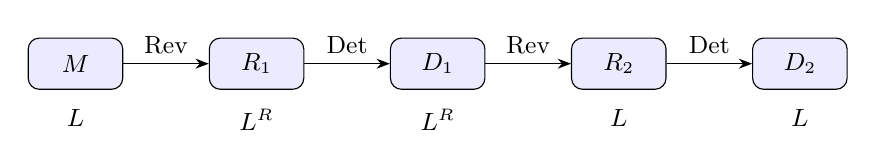
\begin{tikzpicture}[>=Stealth, every node/.style={font=\small},
        box/.style={draw,rounded corners,fill=blue!8,minimum width=1.2cm,
        minimum height=0.65cm}]
      \node[box] (m) at (0,0) {$M$};
      \node[box] (r1) at (2.3,0) {$R_1$};
      \node[box] (d1) at (4.6,0) {$D_1$};
      \node[box] (r2) at (6.9,0) {$R_2$};
      \node[box] (d2) at (9.2,0) {$D_2$};
      \draw[->] (m) -- node[above] {Rev} (r1);
      \draw[->] (r1) -- node[above] {Det} (d1);
      \draw[->] (d1) -- node[above] {Rev} (r2);
      \draw[->] (r2) -- node[above] {Det} (d2);
      \node[below=0.12cm of m] {$L$};
      \node[below=0.12cm of r1] {$L^R$};
      \node[below=0.12cm of d1] {$L^R$};
      \node[below=0.12cm of r2] {$L$};
      \node[below=0.12cm of d2] {$L$};
    \end{tikzpicture}
  \end{center}
  \pause
  \begin{itemize}
    \item \textbf{Rev:} reverse all edges; the old accepting states form the
      initial set, and the old start is the sole accepting state.
      A fresh start with epsilon edges can implement the initial set.
    \item \textbf{Det:} keep only reachable subsets, including $\emptyset$
      if reached. An empty initial set becomes start state $\emptyset$.
    \item Starting with a DFA $M$, the final $D_2$ is the minimal complete DFA.
  \end{itemize}
  \begin{alertblock}{Elegant does not mean asymptotically faster}
    Intermediate subset automata may be exponentially large. This is not
    a replacement for Hopcroft's worst-case $O(n\log n)$ guarantee.
  \end{alertblock}
\end{frame}

\begin{frame}{Why Double Reversal Produces a Minimal DFA}
  \small
  \begin{block}{Key lemma}
    If $A$ is a reachable DFA, then $\operatorname{Det}(\operatorname{Rev}(A))$
    is minimal: its distinct reachable subset states are distinguishable.
  \end{block}
  \pause
  Take distinct subsets $S,T$ and a state $q$ belonging to exactly one of them.
  Since $A$ is reachable, choose $u$ with $\delta_A^*(q_0,u)=q$.
  In the reversed machine, a path labeled $u^R$ leads from a state $r$
  to $q_0$ exactly when $A$ has a path labeled $u$ from $q_0$ to $r$.
  Determinism makes that endpoint uniquely $q$.
  \[
    u^R\text{ is accepted from subset }S\quad\Longleftrightarrow\quad q\in S.
  \]
  Thus $u^R$ distinguishes $S$ and $T$. All output states are reachable,
  so the DFA is minimal.
  \pause
  \begin{block}{Apply the lemma to the second determinization}
    The first determinization produces a reachable DFA $D_1$ for $L^R$.
    The lemma makes $D_2$ minimal, and reversing twice restores $L$.
    The argument also handles the one-state automata for the empty language.
  \end{block}
  Further perspective:~\cite{brzozowski-duality}.
\end{frame}

\begin{frame}{An Exponential Gap in Description Size}
  \small
  Fix $k\ge1$. Let $L_k$ contain binary words whose $k$th symbol from the
  right is $1$ (words shorter than $k$ are rejected).
  \begin{block}{An NFA with $k+1$ states}
    At $q_0$, loop on $0,1$ and also allow $q_0\xrightarrow{1}q_1$.
    For $1\le i<k$, let either symbol move $q_i$ to $q_{i+1}$.
    Only $q_k$ accepts, and it has no outgoing transitions. Guess the
    relevant $1$, then require exactly $k-1$ more symbols.
  \end{block}
  \pause
  \textbf{Every DFA needs at least $2^k$ states.} Take two distinct length-$k$
  words $x,y$ and a position $j$ from the left where they differ. Append
  $0^{j-1}$ to both. Their original $j$th symbols are now $k$th from the
  right, so exactly one extended word belongs to $L_k$.
  All $2^k$ prefixes must therefore lead to distinct states.
  \pause
  \par\smallskip
  A DFA storing the last $k$ bits, initially padded with zeros, attains this
  bound. Hence nondeterminism can save exponentially many states without
  recognizing any additional languages.
\end{frame}

\begin{frame}{Fooling Sets: A Lower Bound That Works for NFAs}
  \small
  \begin{block}{A strong fooling-set criterion~\cite{glaister-shallit}}
    Suppose pairs $(x_i,y_i)$, $1\le i\le r$, satisfy
    \[
      x_i y_i\in L\quad\text{for every }i,\qquad
      x_i y_j\notin L\quad\text{whenever }i\ne j.
    \]
    Then every $\varepsilon$-NFA for $L$ has at least $r$ states.
  \end{block}
  \pause
  \textbf{Proof by splicing paths.} Choose an accepting path for each $x_i y_i$,
  and let $p_i$ be its state at the boundary after $x_i$ and before $y_i$.
  If $p_i=p_j$, follow the first path's $x_i$ portion and the second path's
  $y_j$ portion. This accepts the forbidden word $x_i y_j$.
  Therefore all $p_i$ are distinct. Epsilon moves do not affect the splice.
  \pause
  \begin{alertblock}{Do not confuse DFA and NFA lower bounds}
    Distinguishable prefixes directly lower-bound DFA states. An NFA can
    reach many states after one prefix, so that argument alone does not
    lower-bound its state count. The path-splicing argument supplies the
    additional requirement here.
  \end{alertblock}
\end{frame}

\begin{frame}{Solved Challenge: Can Nondeterminism Shorten a Chain?}
  \small
  For $L_m=\{a^m\}$, $m\ge1$, use pairs
  \[
    (x_i,y_i)=(a^i,a^{m-i}),\qquad 0\le i\le m.
  \]
  Each diagonal word is $a^m$. A cross word has length $m+i-j\ne m$,
  so every NFA needs at least $m+1$ states by the fooling-set criterion.
  \pause
  A chain attains the bound. For $m=3$:
  \begin{center}
    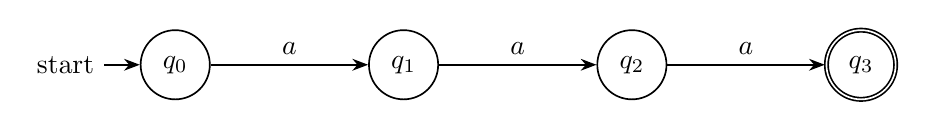
\begin{tikzpicture}[->,>=Stealth,auto,semithick,node distance=2cm]
      \node[state,initial] (q0) {$q_0$};
      \node[state,right=of q0] (q1) {$q_1$};
      \node[state,right=of q1] (q2) {$q_2$};
      \node[state,accepting,right=of q2] (q3) {$q_3$};
      \path (q0) edge node {$a$} (q1)
        (q1) edge node {$a$} (q2)
        (q2) edge node {$a$} (q3);
    \end{tikzpicture}
  \end{center}
  \pause
  \begin{block}{Why a complete DFA needs one more state}
    It must explicitly reject inputs longer than $m$, so add a sink.
    The $m+1$ chain states have different accepted continuations
    $\{a^{m-i}\}$; the sink has none. All are reachable and pairwise
    distinguishable. Thus the minima are $m+1$ for NFAs and $m+2$ for
    complete DFAs, not an exponential difference in this example.
  \end{block}
\end{frame}

\begin{frame}{Algorithmic Costs: Representation Matters}
  \small
  Let $m\ge1$ be input length, $k$ the NFA state count, $e$ its number of
  labeled edges, and $n$ the supplied DFA state count. Fix a finite alphabet.
  \begin{itemize}
    \item \textbf{DFA simulation:} $O(m)$ time with constant-time transition
      lookup and one current-state identifier.
    \item \textbf{NFA set simulation:} $O(m(k+e))$ time by scanning outgoing
      edges and computing closure with visited states; $O(k)$ working space
      beyond the stored automaton. No explicit enumeration of paths is needed.
    \pause
    \item \textbf{Determinization:} up to $2^k$ subset states. This is
      preprocessing; it may be too large even when direct simulation is easy.
    \item \textbf{Table filling:} a dependency-queue implementation achieves
      $O(n^2)$ time and space. Repeatedly rescanning the whole pair table can
      take longer; the classroom pseudocode alone does not ensure this bound.
    \item \textbf{Hopcroft minimization:} $O(n\log n)$ time for a fixed
      alphabet, using efficient partition refinement; see~\cite{hopcroft}.
  \end{itemize}
  \begin{alertblock}{Do not transfer the DFA theorem to NFAs}
    The pair-merging algorithm and uniqueness theorem here concern DFAs.
    Determinizing and minimizing gives a minimal DFA, not a minimal NFA.
  \end{alertblock}
\end{frame}

\subsection{References}

\begin{frame}{References: Textbook Challenge Sources}
  \small
  \setbeamertemplate{bibliography item}[text]
  \begin{thebibliography}{9}
    \bibitem[PSU13]{addition-source}
      Tim Sheard, Portland State University, CS~311, Fall 2013,
      \href{https://web.cecs.pdx.edu/~sheard/course/CS311/Fall2013/homework/assign2.pdf}
      {Homework 2}, problem~6, identifying the binary-addition exercise
      as Sipser~1.32.
    \bibitem[UCSD08]{comparison-source}
      UC San Diego, CSE~105, Fall 2008,
      \href{https://cseweb.ucsd.edu/classes/fa08/cse105/hw1.pdf}
      {Homework 1}, problem~5: binary comparison with a gap of two,
      described there as an extension of Sipser~1.34 (2nd ed.).
  \end{thebibliography}
  \begin{block}{Attribution and conventions}
    The challenge statements above are adapted, and the worked solutions
    are written for this slide set. Exercise numbers refer to these
    verified handouts, not to an assumed numbering in every edition.
    The slides explicitly specify reading direction, leading zeros,
    and the value of an empty row.
  \end{block}
  The remaining practice problems are original textbook-style exercises
  aligned with Linz and Sipser, not claimed to be copied book exercises.
\end{frame}

\begin{frame}{References: Optional Automata Results}
  \small
  \setbeamertemplate{bibliography item}[text]
  \begin{thebibliography}{9}
    \bibitem[B14]{brzozowski-duality}
      Filippo Bonchi, Marcello M. Bonsangue, Helle H. Hansen,
      Prakash Panangaden, Jan J. M. M. Rutten, and Alexandra Silva,
      \href{https://doi.org/10.1145/2490818}
      {\emph{Algebra-Coalgebra Duality in Brzozowski's Minimization Algorithm}},
      ACM Transactions on Computational Logic, 15(1), article~3, 2014.
    \bibitem[GS96]{glaister-shallit}
      Ian Glaister and Jeffrey Shallit,
      \href{https://doi.org/10.1016/0020-0190(96)00095-6}
      {\emph{A Lower Bound Technique for the Size of Nondeterministic
      Finite Automata}}, Information Processing Letters, 59(2),
      pp.\ 75--77, 1996.
  \end{thebibliography}
  These sources support optional enrichment beyond the basic textbook
  conversion and minimization procedures. The slides include proof
  sketches so that the results can be used without reading the full papers.
\end{frame}

\begin{frame}{References and Suggested Teaching Route}
  \footnotesize
  \setbeamertemplate{bibliography item}[text]
  \begin{thebibliography}{9}
    \bibitem[LR23]{linz}
      Peter Linz and Susan H. Rodger,
      \emph{An Introduction to Formal Languages and Automata}, 7th ed.,
      Jones \& Bartlett Learning, 2023. Chapter~2: finite automata,
      equivalence, and state reduction.
    \bibitem[S13]{sipser}
      Michael Sipser, \emph{Introduction to the Theory of Computation},
      3rd ed., Cengage, 2013. Sections~1.1--1.2: finite automata and
      nondeterminism. See also his
      \href{https://ocw.mit.edu/courses/18-404j-theory-of-computation-fall-2020/pages/lecture-notes/}
      {MIT 18.404J lecture notes} (2020).
    \bibitem[H71]{hopcroft}
      John Hopcroft,
      \href{https://www.cs.cmu.edu/~cdm/resources/Hopcroft1971.pdf}
      {\emph{An $n\log n$ Algorithm for Minimizing States in a Finite Automaton}},
      Stanford technical report STAN-CS-71-190, 1971.
  \end{thebibliography}
  Keep the worked state-design, subset, and marking examples in the main
  lecture. Use the appendix for proof enrichment, additional practice,
  and implementation tradeoffs. Adapted textbook challenges are identified
  explicitly in the source slide; the remaining exercises are original.
\end{frame}

\end{document}
